\section{$\rho_1$ cannot be 4-transposition}

\begin{theorem}
  \label{exclude-1}
  If $\rho_1$ is a 4-transposition, then a generator can be written as a product of other generators, and thus the generating set is not free, and the group is not a sggi.
\end{theorem}

\begin{proof}
We will use the method saw in~\ref{method}.

\paragraph{}
First we choose an involution, it this case $\rho_1$. The graph with only this involution is displayed in Figure~\ref{proof-5-1}.

\begin{figure}[H]
  \begin{center}
    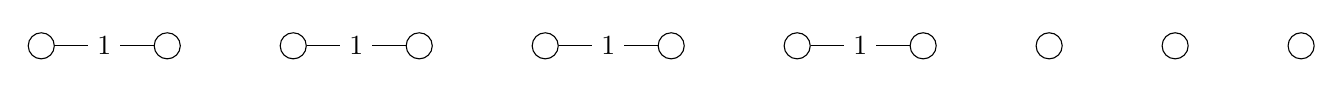
\begin{tikzpicture}[scale=.8]

      \begin{scope}[every node/.style={circle,draw}]
        \node (1)  at (0,0)  {};
        \node (2)  at (2,0)  {};
        \node (3)  at (4,0)  {};
        \node (4)  at (6,0)  {};
        \node (5)  at (8,0)  {};
        \node (6)  at (10,0)  {};
        \node (7)  at (12,0)  {};
        \node (8)  at (14,0)  {};
        \node (9)  at (16,0)  {};
        \node (10) at (18,0)  {};
        \node (11) at (20,0) {};
      \end{scope}

      \begin{scope}[every node/.style={fill=white}]

        \begin{scope}[every edge/.style={draw}]
          \path (1)  edge node {$1$} (2);
          \path (3)  edge node {$1$} (4);
          \path (5)  edge node {$1$} (6);
          \path (7)  edge node {$1$} (8);
        \end{scope}
      \end{scope}

    \end{tikzpicture}
    \caption{}
    \label{proof-5-1}
  \end{center}
\end{figure}

\paragraph{}
Now we will add the involution $\rho_4$. $\rho_1$ and $\rho_4$ must commute. Lemma~\ref{patterns-adding} applies and there are only three possibilities to place the two $\rho_4$ edges.

\paragraph{}
We will now applies the second part of the Method~\ref{method}. For each of those pattern we will continue with the third step. The first part deal with the first pattern, an alternating square $[\rho_1, \rho_4]$, the second part with a single double edge $(\rho_1, \rho_4)$ and the last part with two double edges $(\rho_1, \rho_4)$.

\paragraph{}
\textbf{The alternating square}

\begin{figure}[H]
  \begin{center}
    \begin{tikzpicture}[scale=.8]

      \begin{scope}[every node/.style={circle,draw}]
        \node (1)  at (0,2)  {};
        \node (2)  at (0,0)  {};
        \node (3)  at (2,2)  {};
        \node (4)  at (2,0)  {};
        \node (5)  at (4,0)  {};
        \node (6)  at (6,0)  {};
        \node (7)  at (8,0)  {};
        \node (8)  at (10,0)  {};
        \node (9)  at (12,0)  {};
        \node (10) at (14,0)  {};
        \node (11) at (16,0) {};
      \end{scope}

      \begin{scope}[every node/.style={fill=white}]

        \begin{scope}[every edge/.style={draw}]
          \path (1)  edge node {$1$} (2);
          \path (3)  edge node {$1$} (4);
          \path (5)  edge node {$1$} (6);
          \path (7)  edge node {$1$} (8);
          \path (1)  edge node {$4$} (3);
          \path (2)  edge node {$4$} (4);
        \end{scope}
      \end{scope}

    \end{tikzpicture}
    \caption{}
    \label{proof-5-2}
  \end{center}
\end{figure}

\paragraph{}
Now we will apply the third part of the method and try to form a connected graph by adding some edge. First we will try to extend the alternating square to a sequence. Then we will place the two $\rho_0$ edges. Finally we will add some $\rho_2$ edge to link everything.

\paragraph{}
If $\rho_4$ forms an alternating square with $\rho_1$, it must be adjacent to an other alternating square by Corollary~\ref{continue-alternating-square}. The possibilities are $[\rho_1, \rho_3]$ or $[\rho_2, \rho_4]$ by Proposition~\ref{adjacent-squares}. But the last one is impossible because $\rho_4$ is a 2-transposition by Lemma~\ref{exclude-0}.

\begin{figure}[H]
  \begin{center}
    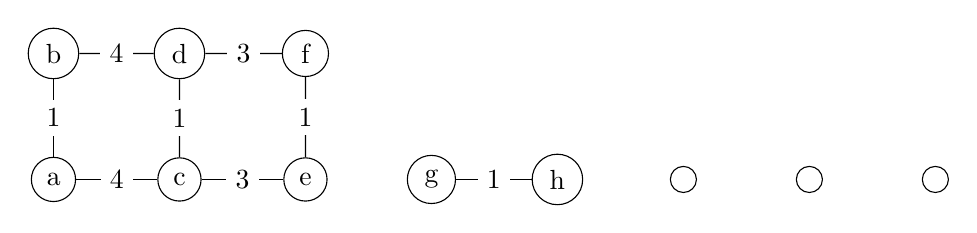
\begin{tikzpicture}[scale=.8]

      \begin{scope}[every node/.style={circle,draw}]
        \node (1)  at (0,2)  {b};
        \node (2)  at (0,0)  {a};
        \node (3)  at (2,2)  {d};
        \node (4)  at (2,0)  {c};
        \node (5)  at (4,2)  {f};
        \node (6)  at (4,0)  {e};
        \node (7)  at (6,0)  {g};
        \node (8)  at (8,0)  {h};
        \node (9)  at (10,0) {};
        \node (10) at (12,0) {};
        \node (11) at (14,0) {};
      \end{scope}

      \begin{scope}[every node/.style={fill=white}]

        \begin{scope}[every edge/.style={draw}]
          \path (1)  edge node {$1$} (2);
          \path (3)  edge node {$1$} (4);
          \path (5)  edge node {$1$} (6);
          \path (7)  edge node {$1$} (8);
          \path (3)  edge node {$3$} (5);
          \path (4)  edge node {$3$} (6);
          \path (1)  edge node {$4$} (3);
          \path (2)  edge node {$4$} (4);
        \end{scope}
      \end{scope}

    \end{tikzpicture}
    \caption{}
    \label{proof-5-3}
  \end{center}
\end{figure}

\paragraph{}
The sequence of squares cannot be extended to the right because two extra alternating squares are needed by Corollary~\ref{parity-sequence-squares}. If the sequence is linear, two additional $\rho_1$ edge would be used. There is only one remaining $\rho_1$ edge, therefore it is not possible to continue linearly. Also it is not possible to place the only rotation pattern found in Lemma~\ref{rotation-pattern}. The sequence cannot be extended on the right.

\paragraph{}
If the sequence is extended to the left, an alternating square $[\rho_1, \rho_3]$ will be built. This uses the last $\rho_1$ edge and the last two $\rho_3$ edges. After that, only 2 $\rho_0$ edges and 2 or 4 $\rho_2$ edges remain but they cannot form a connected graph.

\paragraph{}
The sequence of alternating squares cannot be extended neither on the left nor on the right. Now we will place the $\rho_0$ edges.

\paragraph{}
By Lemma~\ref{adjacent-must-not-commute} $\rho_0$ and $\rho_1$ must not commute. Thus a $\rho_0$ edge must share a vertex with a $\rho_1$ edge. By Lemma~\ref{0-4-no-share}, the edges of involutions $\rho_0$ and $\rho_4$ cannot share a vertex. So the $\rho_0$ edge cannot be linked to the vertices $a, b, c$ or $d$ of Figure~\ref{proof-5-3}. Also, they cannot be connected to the vertices $e$ or $f$ because it would form an alternating square. But it is in contradiction with the fact that the sequence of alternating square cannot be extended.

\paragraph{}
There are 5 acceptable vertices to place the two $\rho_0$ edges. They use 4 vertices. If one $\rho_0$ edge is connected to $g$ and the other is connected to $h$, it is impossible to make a connected graph. This component cannot be linked at all. The $g$ and $h$ vertices cannot be connected by at the same time. Hence no $\rho_1$ edge are available to connect those $\rho_0$ edge.\footnote{Complete?}

\paragraph{}
Thus only $g$ or $h$ can be used to connect a $\rho_0$ edge. But both cases are isomorphic. Thus there is only one possibility for the graph. It is displayed in Figure~\ref{proof-5-4}.

\begin{figure}[H]
  \begin{center}
    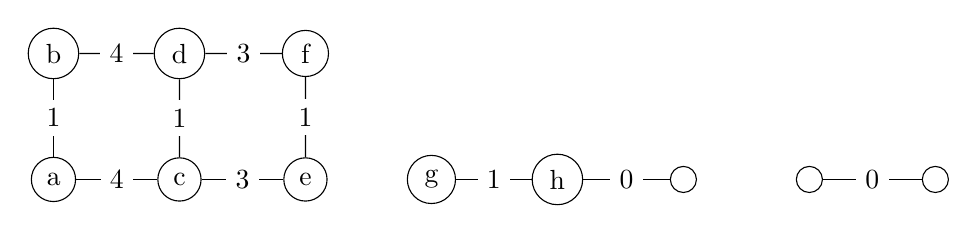
\begin{tikzpicture}[scale=.8] \ref{no-extremity-connection-to-square}

      \begin{scope}[every node/.style={circle,draw}]
        \node (1)  at (0,2)  {b};
        \node (2)  at (0,0)  {a};
        \node (3)  at (2,2)  {d};
        \node (4)  at (2,0)  {c};
        \node (5)  at (4,2)  {f};
        \node (6)  at (4,0)  {e};
        \node (7)  at (6,0)  {g};
        \node (8)  at (8,0)  {h};
        \node (9)  at (10,0) {};
        \node (10) at (12,0) {};
        \node (11) at (14,0) {};
      \end{scope}

      \begin{scope}[every node/.style={fill=white}]

        \begin{scope}[every edge/.style={draw}]
          \path (8)  edge node {$0$} (9);
          \path (10) edge node {$0$} (11);
          \path (1)  edge node {$1$} (2);
          \path (3)  edge node {$1$} (4);
          \path (5)  edge node {$1$} (6);
          \path (7)  edge node {$1$} (8);
          \path (3)  edge node {$3$} (5);
          \path (4)  edge node {$3$} (6);
          \path (1)  edge node {$4$} (3);
          \path (2)  edge node {$4$} (4);
        \end{scope}
      \end{scope}

    \end{tikzpicture}
    \caption{}
    \label{proof-5-4}
  \end{center}
\end{figure}

\paragraph{}
We will place the last remaining edge: $\rho_2$.

\paragraph{}
By Corollary~\ref{sequence-connection}, only a single edge can be connected to the sequence of alternating squares. And this edge cannot be connected to vertices $a,b,c,d$ due to Proposition~\ref{square-connection}. It must be connected to vertices $e$ or $f$ and it must be a $\rho_2$ edge by the same Lemma. But both case are isomorphic so only one is kept.

\paragraph{}
The only available vertex to connect the other end of this $\rho_2$ edge is the point $g$.

\begin{figure}[H]
  \begin{center}
    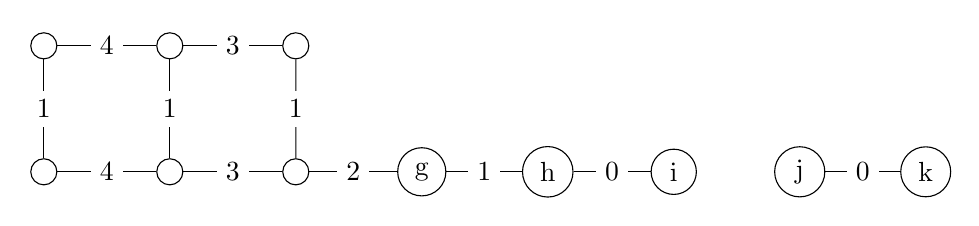
\begin{tikzpicture}[scale=.8]

      \begin{scope}[every node/.style={circle,draw}]
        \node (1)  at (0,2)  {};
        \node (2)  at (0,0)  {};
        \node (3)  at (2,2)  {};
        \node (4)  at (2,0)  {};
        \node (5)  at (4,2)  {};
        \node (6)  at (4,0)  {};
        \node (7)  at (6,0)  {g};
        \node (8)  at (8,0)  {h};
        \node (9)  at (10,0)  {i};
        \node (10) at (12,0)  {j};
        \node (11) at (14,0) {k};
      \end{scope}

      \begin{scope}[every node/.style={fill=white}]

        \begin{scope}[every edge/.style={draw}]
          \path (8)  edge node {$0$} (9);
          \path (10) edge node {$0$} (11);
          \path (1)  edge node {$1$} (2);
          \path (3)  edge node {$1$} (4);
          \path (5)  edge node {$1$} (6);
          \path (7)  edge node {$1$} (8);
          \path (6)  edge node {$2$} (7);
          \path (3)  edge node {$3$} (5);
          \path (4)  edge node {$3$} (6);
          \path (1)  edge node {$4$} (3);
          \path (2)  edge node {$4$} (4);
        \end{scope}
      \end{scope}

    \end{tikzpicture}
    \caption{}
  \end{center}
\end{figure}

\paragraph{}
All $\rho_1$ edges have been used, so they cannot be used to link the $\rho_0$ edge $(j,k)$. Therefore this edge must be part of an alternating square. This square must include the $\rho_0$ edge $(h,i)$ because it is the only other $\rho_0$ edge. The creation of the square will use two other edge of a given index. Those edge will be $(h,j)$ and $(i,k)$. But the edge $(h,j)$ is adjacent to the $\rho_1$ edge $(g,h)$. Therefore, the index of the other edges of the square must thus be consecutive to $1$. Hence the index of the other involution of the alternating square edges must be $2$. The result can be seen on Figure~\ref{proof-5-5}.

\begin{figure}[H]
  \begin{center}
    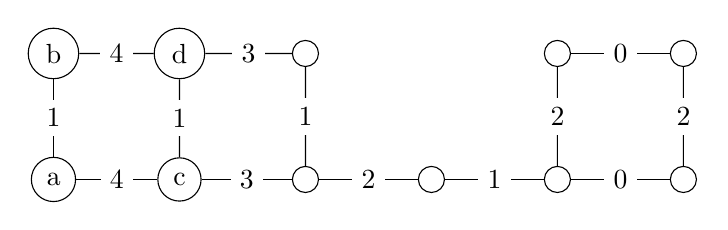
\begin{tikzpicture}[scale=.8]

      \begin{scope}[every node/.style={circle,draw}]
        \node (1)  at (0,2)  {b};
        \node (2)  at (0,0)  {a};
        \node (3)  at (2,2)  {d};
        \node (4)  at (2,0)  {c};
        \node (5)  at (4,2)  {};
        \node (6)  at (4,0)  {};
        \node (7)  at (6,0)  {};
        \node (8)  at (8,2)  {};
        \node (9)  at (8,0)  {};
        \node (10) at (10,2)  {};
        \node (11) at (10,0) {};
      \end{scope}

      \begin{scope}[every node/.style={fill=white}]

        \begin{scope}[every edge/.style={draw}]
          \path (9)  edge node {$0$} (11);
          \path (8)  edge node {$0$} (10);
          \path (1)  edge node {$1$} (2);
          \path (3)  edge node {$1$} (4);
          \path (5)  edge node {$1$} (6);
          \path (7)  edge node {$1$} (9);
          \path (6)  edge node {$2$} (7);
          \path (8)  edge node {$2$} (9);
          \path (10) edge node {$2$} (11);
          \path (3)  edge node {$3$} (5);
          \path (4)  edge node {$3$} (6);
          \path (1)  edge node {$4$} (3);
          \path (2)  edge node {$4$} (4);
        \end{scope}
      \end{scope}

    \end{tikzpicture}
    \caption{}
    \label{proof-5-5}
  \end{center}
\end{figure}

\paragraph{}
The graph is now connected, we enter our last part of the method: adding edges until all of them are placed.

\paragraph{}
There are only 3 $\rho_2$ edges on this graph. A last one must be added to restore parity. There are only two possible places: $(a,b)$ or $(c,d)$. That gives 2 graphs:

\begin{figure}[H]
  \begin{center}
    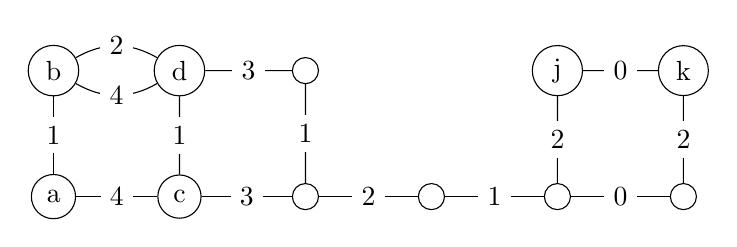
\begin{tikzpicture}[scale=.8]

      \begin{scope}[every node/.style={circle,draw}]
        \node (1)  at (0,2)  {b};
        \node (2)  at (0,0)  {a};
        \node (3)  at (2,2)  {d};
        \node (4)  at (2,0)  {c};
        \node (5)  at (4,2)  {};
        \node (6)  at (4,0)  {};
        \node (7)  at (6,0)  {};
        \node (8)  at (8,2)  {j};
        \node (9)  at (8,0)  {};
        \node (10) at (10,2)  {k};
        \node (11) at (10,0) {};
      \end{scope}

      \begin{scope}[every node/.style={fill=white}]

        \begin{scope}[every edge/.style={draw}]
          \path (9)  edge node {$0$} (11);
          \path (8)  edge node {$0$} (10);
          \path (1)  edge node {$1$} (2);
          \path (3)  edge node {$1$} (4);
          \path (5)  edge node {$1$} (6);
          \path (7)  edge node {$1$} (9);
          \path (1)  edge[bend left=30] node {$2$} (3);
          \path (6)  edge node {$2$} (7);
          \path (8)  edge node {$2$} (9);
          \path (10) edge node {$2$} (11);
          \path (3)  edge node {$3$} (5);
          \path (4)  edge node {$3$} (6);
          \path (1)  edge[bend right=30] node {$4$} (3);
          \path (2)  edge node {$4$} (4);
        \end{scope}
      \end{scope}

    \end{tikzpicture}
    \caption{}
  \end{center}
\end{figure}

\begin{figure}[H]
  \begin{center}
    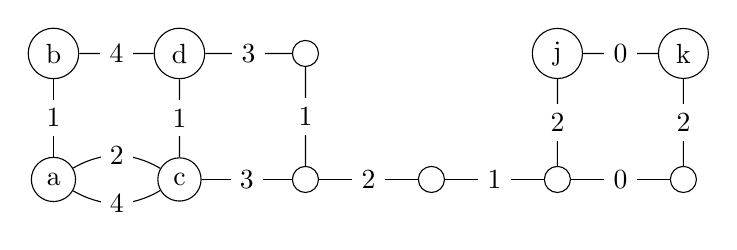
\begin{tikzpicture}[scale=.8]

      \begin{scope}[every node/.style={circle,draw}]
        \node (1)  at (0,2)  {b};
        \node (2)  at (0,0)  {a};
        \node (3)  at (2,2)  {d};
        \node (4)  at (2,0)  {c};
        \node (5)  at (4,2)  {};
        \node (6)  at (4,0)  {};
        \node (7)  at (6,0)  {};
        \node (8)  at (8,2)  {j};
        \node (9)  at (8,0)  {};
        \node (10) at (10,2)  {k};
        \node (11) at (10,0) {};
      \end{scope}

      \begin{scope}[every node/.style={fill=white}]

        \begin{scope}[every edge/.style={draw}]
          \path (9)  edge node {$0$} (11);
          \path (8)  edge node {$0$} (10);
          \path (1)  edge node {$1$} (2);
          \path (3)  edge node {$1$} (4);
          \path (5)  edge node {$1$} (6);
          \path (7)  edge node {$1$} (9);
          \path (2)  edge[bend left=30] node {$2$} (4);
          \path (6)  edge node {$2$} (7);
          \path (8)  edge node {$2$} (9);
          \path (10) edge node {$2$} (11);
          \path (3)  edge node {$3$} (5);
          \path (4)  edge node {$3$} (6);
          \path (1)  edge node {$4$} (3);
          \path (2)  edge[bend right=30] node {$4$} (4);
        \end{scope}
      \end{scope}

    \end{tikzpicture}
    \caption{}
  \end{center}
\end{figure}

\paragraph{}
Those graphs are valid permutation representation graphs but $\rho_3$ is a 2-transposition. To find all possibles sggis, it is needed to try to extend it to a 4-transposition. There are only two possible positions for extra $\rho_3$ edges: between $(a,b)$ and $(j,k)$. That creates two other graphs:

\begin{figure}[H]
  \begin{center}
    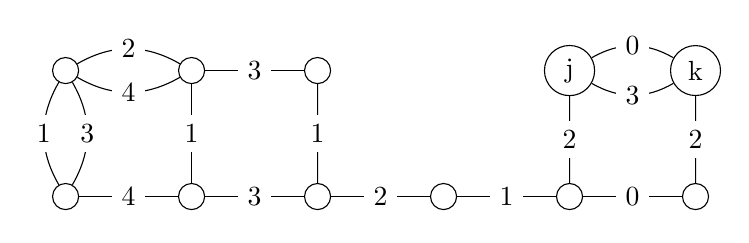
\begin{tikzpicture}[scale=.8]

      \begin{scope}[every node/.style={circle,draw}]
        \node (1)  at (0,2)  {};
        \node (2)  at (0,0)  {};
        \node (3)  at (2,2)  {};
        \node (4)  at (2,0)  {};
        \node (5)  at (4,2)  {};
        \node (6)  at (4,0)  {};
        \node (7)  at (6,0)  {};
        \node (8)  at (8,2)  {j};
        \node (9)  at (8,0)  {};
        \node (10) at (10,2)  {k};
        \node (11) at (10,0) {};
      \end{scope}

      \begin{scope}[every node/.style={fill=white}]

        \begin{scope}[every edge/.style={draw}]
          \path (9)  edge node {$0$} (11);
          \path (8)  edge[bend left=30] node {$0$} (10);
          \path (1)  edge[bend right=30] node {$1$} (2);
          \path (3)  edge node {$1$} (4);
          \path (5)  edge node {$1$} (6);
          \path (7)  edge node {$1$} (9);
          \path (1)  edge[bend left=30] node {$2$} (3);
          \path (6)  edge node {$2$} (7);
          \path (8)  edge node {$2$} (9);
          \path (10) edge node {$2$} (11);
          \path (1)  edge[bend left=30] node {$3$} (2);
          \path (3)  edge node {$3$} (5);
          \path (4)  edge node {$3$} (6);
          \path (8)  edge[bend right=30] node {$3$} (10);
          \path (1)  edge[bend right=30] node {$4$} (3);
          \path (2)  edge node {$4$} (4);
        \end{scope}
      \end{scope}

    \end{tikzpicture}
    \caption{}
  \end{center}
\end{figure}

\begin{figure}[H]
  \begin{center}
    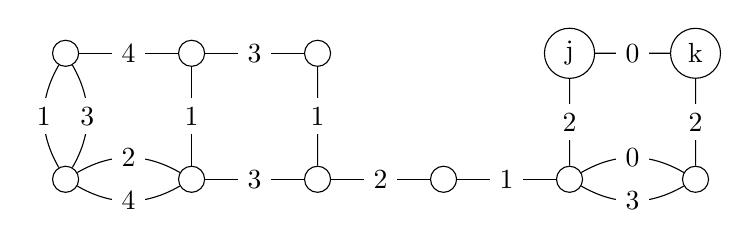
\begin{tikzpicture}[scale=.8]

      \begin{scope}[every node/.style={circle,draw}]
        \node (1)  at (0,2)  {};
        \node (2)  at (0,0)  {};
        \node (3)  at (2,2)  {};
        \node (4)  at (2,0)  {};
        \node (5)  at (4,2)  {};
        \node (6)  at (4,0)  {};
        \node (7)  at (6,0)  {};
        \node (8)  at (8,2)  {j};
        \node (9)  at (8,0)  {};
        \node (10) at (10,2)  {k};
        \node (11) at (10,0) {};
      \end{scope}

      \begin{scope}[every node/.style={fill=white}]

        \begin{scope}[every edge/.style={draw}]
          \path (9)  edge[bend left=30] node {$0$} (11);
          \path (8)  edge node {$0$} (10);
          \path (1)  edge[bend right=30] node {$1$} (2);
          \path (3)  edge node {$1$} (4);
          \path (5)  edge node {$1$} (6);
          \path (7)  edge node {$1$} (9);
          \path (2)  edge[bend left=30] node {$2$} (4);
          \path (6)  edge node {$2$} (7);
          \path (8)  edge node {$2$} (9);
          \path (10) edge node {$2$} (11);
          \path (1)  edge[bend left=30] node {$3$} (2);
          \path (3)  edge node {$3$} (5);
          \path (4)  edge node {$3$} (6);
          \path (9)  edge[bend right=30] node {$3$} (11);
          \path (1)  edge node {$4$} (3);
          \path (2)  edge[bend right=30] node {$4$} (4);
        \end{scope}
      \end{scope}

    \end{tikzpicture}
    \caption{}
  \end{center}
\end{figure}

\paragraph{}
If the $\rho_0 $ and $\rho_3$ edges are removed, the graphs become to following one:

\begin{figure}[H]
  \begin{center}
    \begin{tikzpicture}[scale=.8]

      \begin{scope}[every node/.style={circle,draw}]
        \node (1)  at (0,2)  {};
        \node (2)  at (0,0)  {};
        \node (3)  at (2,2)  {};
        \node (4)  at (2,0)  {};
        \node (5)  at (6,0)  {};
        \node (6)  at (4,0)  {};
        \node (7)  at (8,0)  {};
        \node (8)  at (10,0)  {};
        \node (9)  at (12,0)  {};
        \node (10) at (14,0)  {};
        \node (11) at (16,0) {};
      \end{scope}

      \begin{scope}[every node/.style={fill=white}]

        \begin{scope}[every edge/.style={draw}]
          \path (1)  edge node {$1$} (2);
          \path (3)  edge node {$1$} (4);
          \path (5)  edge node {$1$} (6);
          \path (7)  edge node {$1$} (8);
          \path (1)  edge[bend left=30] node {$2$} (3);
          \path (5)  edge node {$2$} (7);
          \path (8)  edge node {$2$} (9);
          \path (10) edge node {$2$} (11);
          \path (1)  edge[bend right=30] node {$4$} (3);
          \path (2)  edge node {$4$} (4);
        \end{scope}
      \end{scope}

    \end{tikzpicture}
    \caption{}
  \end{center}
\end{figure}

\paragraph{}
But it can be easily seen that $\rho_4 = (\rho_1 \rho_2)^{10}$. Thus none of those four graphs have a free set of generators and so none of then are sggis.

\paragraph{}
\textbf{One double edge}\\
The second possibility is having a double edge $(\rho_1, \rho_4)$. The double edge alone is too small to be used as a starting pattern for the method described in~\ref{method}. By Lemma~\ref{continue-double-edge}, this double edge must be adjacent to some alternating square. The pattern that we will choose include this alternating square. By Proposition~\ref{adjacent-squares}, there are two possibilities for the alternating square: $[\rho_1, \rho_3]$ or $[\rho_2, \rho_4]$. Therefore we have 2 starting patterns.

\paragraph{}
\textit{Alternating square $[\rho_1, \rho_3]$}

\begin{figure}[H]
  \begin{center}
    \begin{tikzpicture}[scale=.8]

      \begin{scope}[every node/.style={circle,draw}]
        \node (1)  at (0,2)  {};
        \node (2)  at (0,0)  {};
        \node (3)  at (2,2)  {};
        \node (4)  at (2,0)  {};
        \node (5)  at (4,0)  {};
        \node (6)  at (6,0)  {};
        \node (7)  at (8,0)  {};
        \node (8)  at (10,0)  {};
        \node (9)  at (12,0)  {};
        \node (10) at (14,0)  {};
        \node (11) at (16,0) {};
      \end{scope}

      \begin{scope}[every node/.style={fill=white}]

        \begin{scope}[every edge/.style={draw}]
          \path (1)  edge[bend right=30] node {$1$} (2);
          \path (3)  edge node {$1$} (4);
          \path (5)  edge node {$1$} (6);
          \path (7)  edge node {$1$} (8);
          \path (1)  edge node {$3$} (3);
          \path (2)  edge node {$3$} (4);
          \path (1)  edge[bend left=30] node {$4$} (2);
        \end{scope}
      \end{scope}

    \end{tikzpicture}
    \caption{}
  \end{center}
\end{figure}

\paragraph{}
By lemma~\ref{adjacent-must-not-commute}, $\rho_0$ and $\rho_1$ must not commute. A $\rho_0$ edge must thus be connected to at least one $\rho_1$ edge. So at least one $\rho_1$ edge must not be part of an alternating square of which $\rho_0$ does not belong.

\paragraph{}
The alternating square cannot be extended to a sequence on the right because this will need two alternating squares by Proposition~\ref{parity-sequence-squares}. If the sequence is linear, the index of the vertical edges is not changed. But adding two squares would require all of the $\rho_1$ edges. None of the horizontal edges of the squares can be an edge of $\rho_0$. Thus, the square cannot be extended to the right by previous statement.

\paragraph{}
The values of the vertical edges must therefore be changed. The horizontal edges of the second square must be $\rho_2$ because the involutions must be adjacent to $\rho_3$ and there is not enough $\rho_4$ edges. Then the new value for vertical edge must be adjacent to $\rho_3$. $\rho_2$ is impossible because it is already used for the horizontal edges. The only remaining possibility is $\rho_4$ but there are no enough remaining edges.

\paragraph{}
If an alternating square is attached on the left, it must be $[\rho_2, \rho_4]$.

\begin{figure}[H]
  \begin{center}
    \begin{tikzpicture}[scale=.8]

      \begin{scope}[every node/.style={circle,draw}]
        \node (1)  at (0,2)  {};
        \node (2)  at (0,0)  {};
        \node (3)  at (2,2)  {};
        \node (4)  at (2,0)  {};
        \node (5)  at (4,0)  {};
        \node (6)  at (6,0)  {};
        \node (7)  at (8,0)  {};
        \node (8)  at (10,0)  {};
        \node (9)  at (-2,2)  {};
        \node (10) at (-2,0)  {};
        \node (11) at (12,0) {};
      \end{scope}

      \begin{scope}[every node/.style={fill=white}]

        \begin{scope}[every edge/.style={draw}]
          \path (1)  edge[bend right=30] node {$1$} (2);
          \path (3)  edge node {$1$} (4);
          \path (5)  edge node {$1$} (6);
          \path (7)  edge node {$1$} (8);
          \path (1)  edge node {$2$} (9);
          \path (2)  edge node {$2$} (10);
          \path (1)  edge node {$3$} (3);
          \path (2)  edge node {$3$} (4);
          \path (1)  edge[bend left=30] node {$4$} (2);
          \path (9)  edge node {$4$} (10);
        \end{scope}
      \end{scope}

    \end{tikzpicture}
    \caption{}
  \end{center}
\end{figure}

\paragraph{}
The two $\rho_0$ edges cannot be placed on any vertex of the left component. If the fixed point is not used to connect the $\rho_0$ edges, the two $\rho_1$ edges must be linked together twice and thus build an alternating square. Then $\rho_0$ and $\rho_1$ commute and that is impossible. Thus the fixed point must be connected by $\rho_0$.

\paragraph{}
The first $\rho_0$ edge must connect the fixed point to a $\rho_1$ edge and the second must connect the two $\rho_1$ edges together.

\begin{figure}[H]
  \begin{center}
    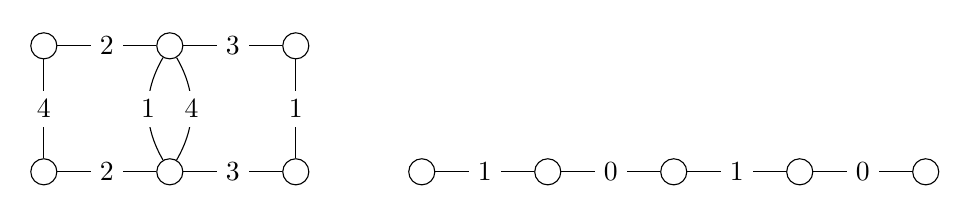
\begin{tikzpicture}[scale=.8]

      \begin{scope}[every node/.style={circle,draw}]
        \node (1)  at (0,2)  {};
        \node (2)  at (0,0)  {};
        \node (3)  at (2,2)  {};
        \node (4)  at (2,0)  {};
        \node (5)  at (4,0)  {};
        \node (6)  at (6,0)  {};
        \node (7)  at (8,0)  {};
        \node (8)  at (10,0)  {};
        \node (9)  at (-2,2)  {};
        \node (10) at (-2,0)  {};
        \node (11) at (12,0) {};
      \end{scope}

      \begin{scope}[every node/.style={fill=white}]

        \begin{scope}[every edge/.style={draw}]
          \path (6)  edge node {$0$} (7);
          \path (8)  edge node {$0$} (11);
          \path (1)  edge[bend right=30] node {$1$} (2);
          \path (3)  edge node {$1$} (4);
          \path (5)  edge node {$1$} (6);
          \path (7)  edge node {$1$} (8);
          \path (1)  edge node {$2$} (9);
          \path (2)  edge node {$2$} (10);
          \path (1)  edge node {$3$} (3);
          \path (2)  edge node {$3$} (4);
          \path (1)  edge[bend left=30] node {$4$} (2);
          \path (9)  edge node {$4$} (10);
        \end{scope}
      \end{scope}

    \end{tikzpicture}
    \caption{}
  \end{center}
\end{figure}

\paragraph{}
Two components must be linked by a $\rho_2$ edge. But the total number of $\rho_2$ edges becomes odd. Another $\rho_2$ must thus be placed. The only possibilities are to double a $\rho_0$ edge. There are two possible graphs:

\begin{figure}[H]
  \begin{center}
    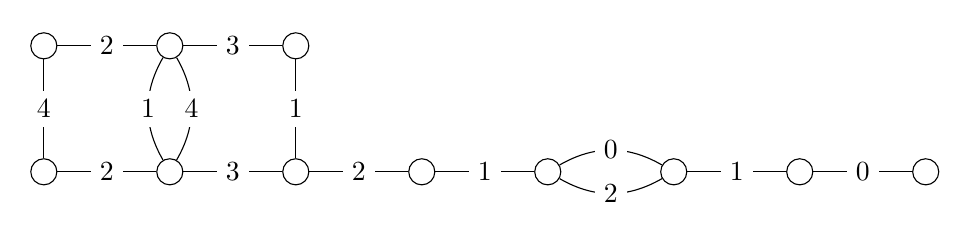
\begin{tikzpicture}[scale=.8]

      \begin{scope}[every node/.style={circle,draw}]
        \node (1)  at (0,2)  {};
        \node (2)  at (0,0)  {};
        \node (3)  at (2,2)  {};
        \node (4)  at (2,0)  {};
        \node (5)  at (4,0)  {};
        \node (6)  at (6,0)  {};
        \node (7)  at (8,0)  {};
        \node (8)  at (10,0)  {};
        \node (9)  at (-2,2)  {};
        \node (10) at (-2,0)  {};
        \node (11) at (12,0) {};
      \end{scope}

      \begin{scope}[every node/.style={fill=white}]

        \begin{scope}[every edge/.style={draw}]
          \path (6)  edge[bend left=30] node {$0$} (7);
          \path (8)  edge node {$0$} (11);
          \path (1)  edge[bend right=30] node {$1$} (2);
          \path (3)  edge node {$1$} (4);
          \path (5)  edge node {$1$} (6);
          \path (7)  edge node {$1$} (8);
          \path (1)  edge node {$2$} (9);
          \path (2)  edge node {$2$} (10);
          \path (4)  edge node {$2$} (5);
          \path (6)  edge[bend right=30] node {$2$} (7);
          \path (1)  edge node {$3$} (3);
          \path (2)  edge node {$3$} (4);
          \path (1)  edge[bend left=30] node {$4$} (2);
          \path (9)  edge node {$4$} (10);
        \end{scope}
      \end{scope}

    \end{tikzpicture}
    \caption{}
  \end{center}
\end{figure}

\begin{figure}[H]
  \begin{center}
    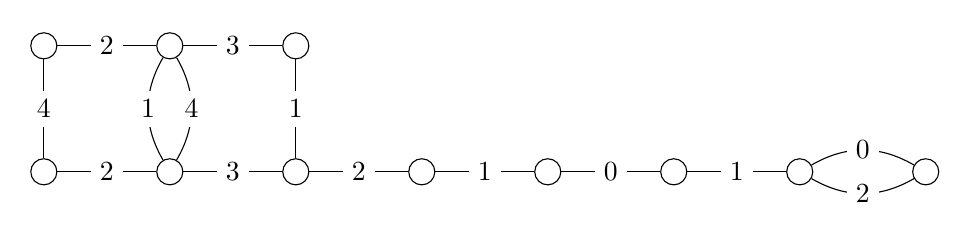
\begin{tikzpicture}[scale=.8]

      \begin{scope}[every node/.style={circle,draw}]
        \node (1)  at (0,2)  {};
        \node (2)  at (0,0)  {};
        \node (3)  at (2,2)  {};
        \node (4)  at (2,0)  {};
        \node (5)  at (4,0)  {};
        \node (6)  at (6,0)  {};
        \node (7)  at (8,0)  {};
        \node (8)  at (10,0)  {};
        \node (9)  at (-2,2)  {};
        \node (10) at (-2,0)  {};
        \node (11) at (12,0) {};
      \end{scope}

      \begin{scope}[every node/.style={fill=white}]

        \begin{scope}[every edge/.style={draw}]
          \path (6)  edge node {$0$} (7);
          \path (8)  edge[bend left=30] node {$0$} (11);
          \path (1)  edge[bend right=30] node {$1$} (2);
          \path (3)  edge node {$1$} (4);
          \path (5)  edge node {$1$} (6);
          \path (7)  edge node {$1$} (8);
          \path (1)  edge node {$2$} (9);
          \path (2)  edge node {$2$} (10);
          \path (4)  edge node {$2$} (5);
          \path (8)  edge[bend right=30] node {$2$} (11);
          \path (1)  edge node {$3$} (3);
          \path (2)  edge node {$3$} (4);
          \path (1)  edge[bend left=30] node {$4$} (2);
          \path (9)  edge node {$4$} (10);
        \end{scope}
      \end{scope}

    \end{tikzpicture}
    \caption{}
  \end{center}
\end{figure}

\paragraph{}
In those graphs, if the $\rho_4$ edge is removed, the generated group is 2-transitive\footnote{TO DO} and thus primitive. By looking at the size of the subgroups, it is possible to deduce that the generated group is $A_{11}$\footnote{Missing the case where no other square are attached}.

\paragraph{}
\textit{Alternating square $[\rho_2,\rho_4]$}

\begin{figure}[H]
  \begin{center}
    \begin{tikzpicture}[scale=.8]

      \begin{scope}[every node/.style={circle,draw}]
        \node (1)  at (0,2)  {};
        \node (2)  at (0,0)  {};
        \node (3)  at (2,2)  {};
        \node (4)  at (2,0)  {};
        \node (5)  at (6,0)  {};
        \node (6)  at (4,0)  {};
        \node (7)  at (10,0)  {};
        \node (8)  at (8,0)  {};
        \node (9)  at (12,0)  {};
        \node (10) at (14,0)  {};
        \node (11) at (16,0) {};
      \end{scope}

      \begin{scope}[every node/.style={fill=white}]

        \begin{scope}[every edge/.style={draw}]
          \path (1)  edge[bend right=30] node {$1$} (2);
          \path (5)  edge node {$1$} (6);
          \path (7)  edge node {$1$} (8);
          \path (9)  edge node {$1$} (10);
          \path (1)  edge node {$2$} (3);
          \path (2)  edge node {$2$} (4);
          \path (1)  edge[bend left=30] node {$4$} (2);
          \path (3)  edge node {$4$} (4);
        \end{scope}
      \end{scope}

    \end{tikzpicture}
    \caption{}
  \end{center}
\end{figure}

\paragraph{}
Either two extra alternating squares can be added or this alternating square can be linked to some other component.

\paragraph{}
In the first case, it is impossible to add another alternating square to right of this sequence.

\paragraph{}
The alternating square can however be extended to the left by a $[\rho_1, \rho_3]$ edge but then it can be reduced to the $[\rho_1, \rho_3]$ case.

\paragraph{}
The only remaining possibility is to link to square to the rest of the graph with a single edge. A $\rho_3$ edge must be used. It cannot be connected to a $\rho_1$ edge an alternating square should be built but that is impossible. The only possibility is to link it to the fixed point.

\begin{figure}[H]
  \begin{center}
    \begin{tikzpicture}[scale=.8]

      \begin{scope}[every node/.style={circle,draw}]
        \node (1)  at (0,2)  {};
        \node (2)  at (0,0)  {};
        \node (3)  at (2,2)  {};
        \node (4)  at (2,0)  {};
        \node (5)  at (8,0)  {};
        \node (6)  at (6,0)  {};
        \node (7)  at (12,0)  {};
        \node (8)  at (10,0)  {};
        \node (9)  at (14,0)  {};
        \node (10) at (16,0)  {};
        \node (11) at (4,0) {};
      \end{scope}

      \begin{scope}[every node/.style={fill=white}]

        \begin{scope}[every edge/.style={draw}]
          \path (1)  edge[bend right=30] node {$1$} (2);
          \path (5)  edge node {$1$} (6);
          \path (7)  edge node {$1$} (8);
          \path (9)  edge node {$1$} (10);
          \path (1)  edge node {$2$} (3);
          \path (2)  edge node {$2$} (4);
          \path (4)  edge node {$3$} (11);
          \path (1)  edge[bend left=30] node {$4$} (2);
          \path (3)  edge node {$4$} (4);
        \end{scope}
      \end{scope}

    \end{tikzpicture}
    \caption{}
  \end{center}
\end{figure}

\paragraph{}
Two $\rho_0$ edges must still be placed and they must not commute with $\rho_1$. Thus at least one edge must link two $\rho_1$ involutions. And the other $\rho_0$ edge must link the two other $\rho_1$ edges.

\begin{figure}[H]
  \begin{center}
    \begin{tikzpicture}[scale=.8]

      \begin{scope}[every node/.style={circle,draw}]
        \node (1)  at (0,2)  {};
        \node (2)  at (0,0)  {};
        \node (3)  at (2,2)  {};
        \node (4)  at (2,0)  {};
        \node (5)  at (8,0)  {};
        \node (6)  at (6,0)  {};
        \node (7)  at (12,0)  {};
        \node (8)  at (10,0)  {};
        \node (9)  at (14,0)  {};
        \node (10) at (16,0)  {};
        \node (11) at (4,0) {};
      \end{scope}

      \begin{scope}[every node/.style={fill=white}]

        \begin{scope}[every edge/.style={draw}]
          \path (5)  edge node {$0$} (8);
          \path (7)  edge node {$0$} (9);
          \path (1)  edge[bend right=30] node {$1$} (2);
          \path (5)  edge node {$1$} (6);
          \path (7)  edge node {$1$} (8);
          \path (9)  edge node {$1$} (10);
          \path (1)  edge node {$2$} (3);
          \path (2)  edge node {$2$} (4);
          \path (4)  edge node {$3$} (11);
          \path (1)  edge[bend left=30] node {$4$} (2);
          \path (3)  edge node {$4$} (4);
        \end{scope}
      \end{scope}

    \end{tikzpicture}
    \caption{}
  \end{center}
\end{figure}

\paragraph{}
Since all $\rho_4$ edge have been used and since no $\rho_2$ can be connected to the alternating square, a $\rho_2$ edge must be used to connect the two components together.

\begin{figure}[H]
  \begin{center}
    \begin{tikzpicture}[scale=.8]

      \begin{scope}[every node/.style={circle,draw}]
        \node (1)  at (0,2)  {};
        \node (2)  at (0,0)  {};
        \node (3)  at (2,2)  {};
        \node (4)  at (2,0)  {};
        \node (5)  at (8,0)  {};
        \node (6)  at (6,0)  {};
        \node (7)  at (12,0)  {};
        \node (8)  at (10,0)  {};
        \node (9)  at (14,0)  {};
        \node (10) at (16,0)  {};
        \node (11) at (4,0) {};
      \end{scope}

      \begin{scope}[every node/.style={fill=white}]

        \begin{scope}[every edge/.style={draw}]
          \path (5)  edge node {$0$} (8);
          \path (7)  edge node {$0$} (9);
          \path (1)  edge[bend right=30] node {$1$} (2);
          \path (5)  edge node {$1$} (6);
          \path (7)  edge node {$1$} (8);
          \path (9)  edge node {$1$} (10);
          \path (1)  edge node {$2$} (3);
          \path (2)  edge node {$2$} (4);
          \path (11)  edge node {$2$} (6);
          \path (4)  edge node {$3$} (11);
          \path (1)  edge[bend left=30] node {$4$} (2);
          \path (3)  edge node {$4$} (4);
        \end{scope}
      \end{scope}

    \end{tikzpicture}
    \caption{}
  \end{center}
\end{figure}

\paragraph{}
The $\rho_3$ involution is currently odd. An extra $\rho_3$ edge must be placed. The only possibility is to triple the double edge. The missing $\rho_2$ edge must then be placed such that a $\rho_0$ edge is doubled. There are two graphs:


\begin{figure}[H]
  \begin{center}
    \begin{tikzpicture}[scale=.8]

      \begin{scope}[every node/.style={circle,draw}]
        \node (1)  at (0,2)  {};
        \node (2)  at (0,0)  {};
        \node (3)  at (2,2)  {};
        \node (4)  at (2,0)  {};
        \node (5)  at (8,0)  {};
        \node (6)  at (6,0)  {};
        \node (7)  at (12,0)  {};
        \node (8)  at (10,0)  {};
        \node (9)  at (14,0)  {};
        \node (10) at (16,0)  {};
        \node (11) at (4,0) {};
      \end{scope}

      \begin{scope}[every node/.style={fill=white}]

        \begin{scope}[every edge/.style={draw}]
          \path (5)  edge[bend left=30] node {$0$} (8);
          \path (7)  edge node {$0$} (9);
          \path (1)  edge[bend right=40] node {$1$} (2);
          \path (5)  edge node {$1$} (6);
          \path (7)  edge node {$1$} (8);
          \path (9)  edge node {$1$} (10);
          \path (1)  edge node {$2$} (3);
          \path (2)  edge node {$2$} (4);
          \path (5)  edge[bend right=30] node {$2$} (8);
          \path (11) edge node {$2$} (6);
          \path (1)  edge node {$3$} (2);
          \path (4)  edge node {$3$} (11);
          \path (1)  edge[bend left=40] node {$4$} (2);
          \path (3)  edge node {$4$} (4);
        \end{scope}
      \end{scope}

    \end{tikzpicture}
    \caption{}
  \end{center}
\end{figure}

\begin{figure}[H]
  \begin{center}
    \begin{tikzpicture}[scale=.8]

      \begin{scope}[every node/.style={circle,draw}]
        \node (1)  at (0,2)  {};
        \node (2)  at (0,0)  {};
        \node (3)  at (2,2)  {};
        \node (4)  at (2,0)  {};
        \node (5)  at (8,0)  {};
        \node (6)  at (6,0)  {};
        \node (7)  at (12,0)  {};
        \node (8)  at (10,0)  {};
        \node (9)  at (14,0)  {};
        \node (10) at (16,0)  {};
        \node (11) at (4,0) {};
      \end{scope}

      \begin{scope}[every node/.style={fill=white}]

        \begin{scope}[every edge/.style={draw}]
          \path (5)  edge node {$0$} (8);
          \path (7)  edge[bend left=30] node {$0$} (9);
          \path (1)  edge[bend right=40] node {$1$} (2);
          \path (5)  edge node {$1$} (6);
          \path (7)  edge node {$1$} (8);
          \path (9)  edge node {$1$} (10);
          \path (1)  edge node {$2$} (3);
          \path (2)  edge node {$2$} (4);
          \path (7)  edge[bend right=30] node {$2$} (9);
          \path (11) edge node {$2$} (6);
          \path (1)  edge node {$3$} (2);
          \path (4)  edge node {$3$} (11);
          \path (1)  edge[bend left=40] node {$4$} (2);
          \path (3)  edge node {$4$} (4);
        \end{scope}
      \end{scope}

    \end{tikzpicture}
    \caption{}
  \end{center}
\end{figure}

\paragraph{}
There are no possibility to convert $\rho_3$ to a 4-transposition in this case.

\paragraph{}
The $\rho_0$ and $\rho_3$ edges can be removed and the obtained graph is the same as those obtained for the alternating square $[\rho_1,\rho_4]$. The consequence are the same: $\rho_4 = (\rho_1\rho_2)^{10}$. The group represented by the previous graphs are therefore not sggi.

\paragraph{}
\textbf{Two double edges}

\paragraph{}
The double edges must be contained into alternating squares by Lemma~\ref{continue-double-edge}. There are two possibilities depending if the two double edge are in the same alternating square or not.

\paragraph{}
If the double edges are placed on the same alternating square, the graph is the following:

\begin{figure}[H]
  \begin{center}
    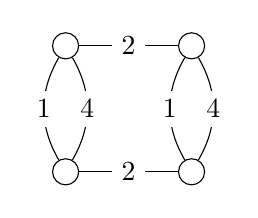
\begin{tikzpicture}[scale=.8]

      \begin{scope}[every node/.style={circle,draw}]
        \node (1)  at (0,2)  {};
        \node (2)  at (0,0)  {};
        \node (3)  at (2,2)  {};
        \node (4)  at (2,0)  {};
      \end{scope}

      \begin{scope}[every node/.style={fill=white}]

        \begin{scope}[every edge/.style={draw}]
          \path (1)  edge[bend right=30] node {$1$} (2);
          \path (3)  edge[bend right=30] node {$1$} (4);
          \path (1)  edge node {$2$} (3);
          \path (2)  edge node {$2$} (4);
          \path (1)  edge[bend left=30] node {$4$} (2);
          \path (3)  edge[bend left=30] node {$4$} (4);
        \end{scope}
      \end{scope}

    \end{tikzpicture}
    \caption{}
  \end{center}
\end{figure}

\paragraph{}
But this situation has already be seen in Figure~\ref{todo} and we proved that no sggi can be made out of this pattern.

\paragraph{}
If the two double edges are place on two different squares. But the possibilities for the squares are limited because each square can only contains one $\rho_4$ edge. The single possibility for the square is $[\rho_1, \rho_3]$ by Proposition~\ref{adjacent-squares}. The graph is the following.

\begin{figure}[H]
  \begin{center}
    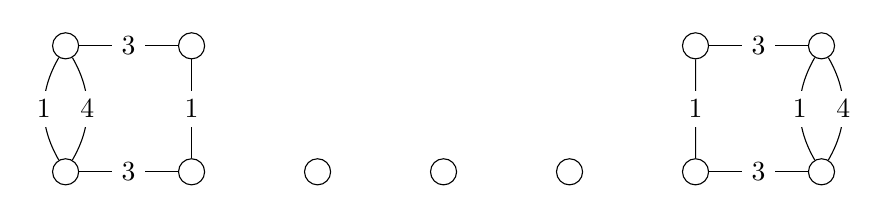
\begin{tikzpicture}[scale=.8]

      \begin{scope}[every node/.style={circle,draw}]
        \node (1)  at (0,2)  {};
        \node (2)  at (0,0)  {};
        \node (3)  at (2,2)  {};
        \node (4)  at (2,0)  {};
        \node (5)  at (8,0)  {};
        \node (6)  at (6,0)  {};
        \node (7)  at (12,0)  {};
        \node (8)  at (10,0)  {};
        \node (9)  at (10,2)  {};
        \node (10) at (12,2)  {};
        \node (11) at (4,0) {};
      \end{scope}

      \begin{scope}[every node/.style={fill=white}]

        \begin{scope}[every edge/.style={draw}]
          \path (1)  edge[bend right=30] node {$1$} (2);
          \path (3)  edge node {$1$} (4);
          \path (8)  edge node {$1$} (9);
          \path (7)  edge[bend left=30] node {$1$} (10);
          \path (1)  edge node {$3$} (3);
          \path (2)  edge node {$3$} (4);
          \path (8)  edge node {$3$} (7);
          \path (9)  edge node {$3$} (10);
          \path (1)  edge[bend left=30] node {$4$} (2);
          \path (7)  edge[bend right=30] node {$4$} (10);
        \end{scope}
      \end{scope}

    \end{tikzpicture}
    \caption{}
  \end{center}
\end{figure}

\paragraph{}
There are only 4 edges available to connect 5 components. Thus every edge must link two different component. Each square must be link by a $\rho_2$ edge by Proposition~\ref{square-connection}.

\begin{figure}[H]
  \begin{center}
    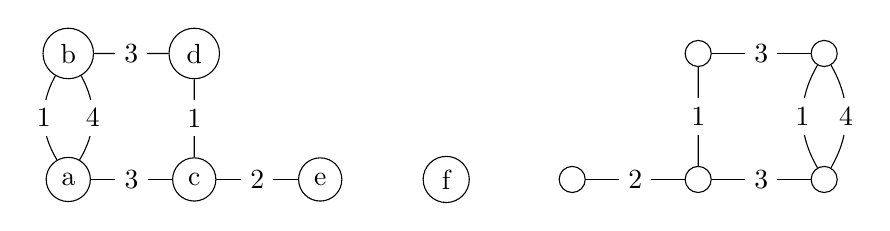
\begin{tikzpicture}[scale=.8]

      \begin{scope}[every node/.style={circle,draw}]
        \node (1)  at (0,2)  {b};
        \node (2)  at (0,0)  {a};
        \node (3)  at (2,2)  {d};
        \node (4)  at (2,0)  {c};
        \node (5)  at (8,0)  {};
        \node (6)  at (6,0)  {f};
        \node (7)  at (12,0)  {};
        \node (8)  at (10,0)  {};
        \node (9)  at (10,2)  {};
        \node (10) at (12,2)  {};
        \node (11) at (4,0) {e};
      \end{scope}

      \begin{scope}[every node/.style={fill=white}]

        \begin{scope}[every edge/.style={draw}]
          \path (1)  edge[bend right=30] node {$1$} (2);
          \path (3)  edge node {$1$} (4);
          \path (8)  edge node {$1$} (9);
          \path (7)  edge[bend left=30] node {$1$} (10);
          \path (4)  edge node {$2$} (11);
          \path (5)  edge node {$2$} (8);
          \path (1)  edge node {$3$} (3);
          \path (2)  edge node {$3$} (4);
          \path (8)  edge node {$3$} (7);
          \path (9)  edge node {$3$} (10);
          \path (1)  edge[bend left=30] node {$4$} (2);
          \path (7)  edge[bend right=30] node {$4$} (10);
        \end{scope}
      \end{scope}

    \end{tikzpicture}
    \caption{}
  \end{center}
\end{figure}

\paragraph{}
But it is not possible to place the $\rho_0$ edges because they will share the vertex $f$ but that is forbidden by Property~\ref{fixed-only-1}

\end{proof}
